\subsection{Designer Preference Model} \label{p5section/model}

The Designer Preference Model is a data-driven intelligent system that learns the user's design style by training and testing over a continuously growing dataset composed of the user's actions and choices while operating EDD. The underlying evolutionary algorithm (EA) uses this model to assess the generated suggestions according to the predicted preference of the designer. This is a complementary assessment to EDD's original fitness function, which evaluates individuals first based on the presence and distribution of spatial and meso-patterns (Figure \ref{p5fig3}), and then based on their degree of adaptation to the user-selected quality-diversity dimensions \citepfifth{p5alvarez2019empowering}. The relevance of the Designer Preference Model gradually increases over EDD's fitness function as long as the model gains confidence in its assessments.

\begin{figure}

\includegraphics[width=\textwidth]{fig3.png}
\caption{A sample room in EDD (a) compose by tiles (b), spatial patterns (c) and meso-patterns (d). Detailed descriptions for these components can be found in~\protect\citepfifth{p5Baldwin2017a}.} \label{p5fig3}
\end{figure}

\begin{figure}
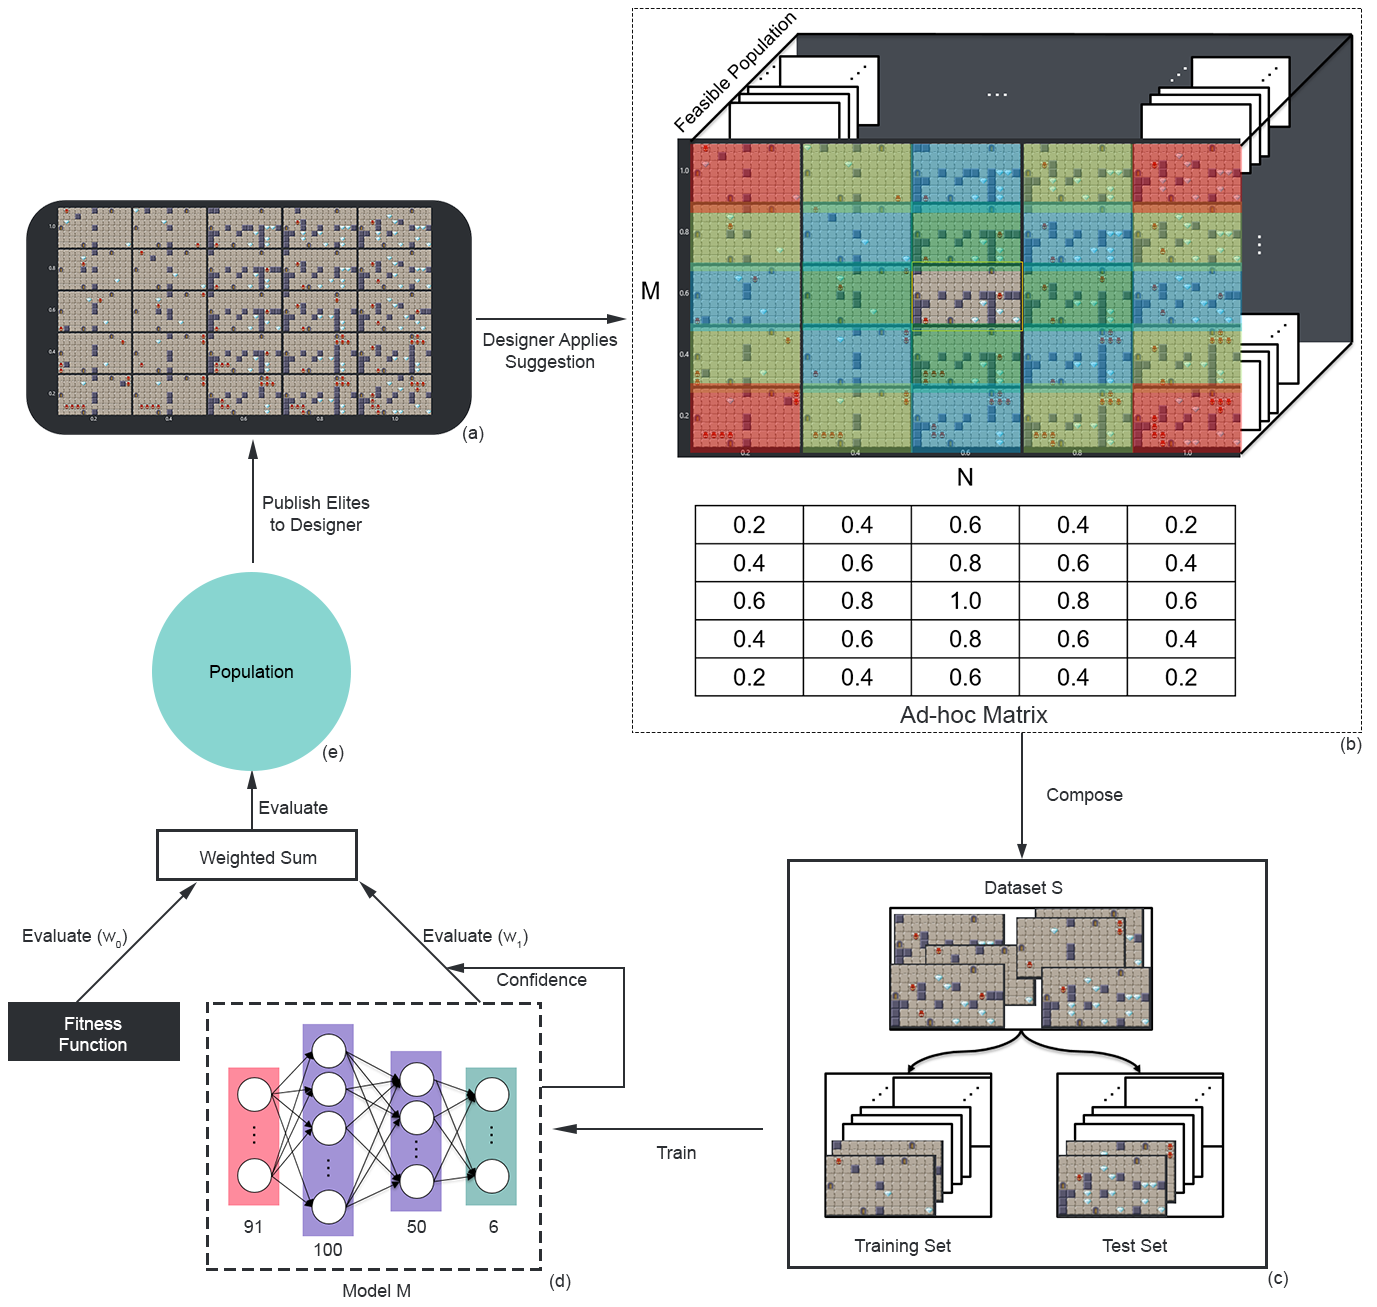
\includegraphics[width=\textwidth]{fig4.png}
\caption{Overview of the Designer Preference Model integrated into the fitness function of EDD. Elites are published and shown to the designer in a grid fashion (a), and once the designer chooses and applies one of the suggestions, an ad-hoc matrix is created based on the position of the selected suggestion to estimate the preference of suggestions (b). The ad-hoc matrix is then applied to all the elites in the grid, and the feasible populations within the EA cells to compose a general dataset $S$ with rooms labeled by the estimated preference. The composed dataset $S$ is then subdivided into a training set (90\%) and test set (10\%), both with the same label distribution (c). The dataset is used to train a model $M$, which is a relatively small neural network, for 20 epochs (d). The  model is then used to evaluate the population of the EA together with the current fitness function in a weighted sum, with the weight of the model $M$ conditioned by the confidence of the network (e).} \label{p5fig4}
\end{figure}

\subsubsection{Model Update and Usage}
The proposed model is a relatively small neural network $M$ with as many input neurons as the number of tiles composing each room, two hidden layers (100 and 50 neurons respectively), and six output neurons, one per each discrete preference value assigned to the individuals by the designer. When the designer starts EDD, the neural network is created with random initialization and without any prior training (i.e. cold start). While the designer creates and modifies rooms, on the background, the EA produces and presents individuals to the designer using the MAP-Elite’s cells (Figure \ref{p5fig2}), while it adapts to the designer’s design. Following a proactive learning approach \citepfifth{p5donmez2008proactive}, anytime the designer chooses one suggestion to replace her current design, a training session is requested for a model $M$ with a dataset $S$ created with the current cells and their populations based on the designer’s chosen suggestion. The loop, depicted in figure \ref{p5fig4}, can be described in the following two steps:

\paragraph{Dataset creation:}

The designer chooses a suggestion to replace her current design, which in turn, requests a training session using all the current individuals (i.e. the elites and the rest of the feasible populations) to create a new dataset to train the model closer to the “actual” preference of the designer. As shown in figure \ref{p5fig4}.b, an ad-hoc matrix is created, based on the position of the applied suggestion, to calculate the estimated preference, starting with the applied suggestion (1.0 preference value), and reducing the preference value by 0.2 per each step that was taken away from the applied suggestion in the matrix until a minimum of 0.0. %Once the ad-hoc matrix is created, all the individuals are given an estimated preference value based on their grid position and are used to compose a general dataset $S$. 

Once all the individuals are given an estimated preference value based on their grid position by the ad-hoc matrix, they are all used to compose a general dataset $S$ where each individual is transformed to match the network input. Finally, we divide the set into a training set (90\%) and test set (10\%) with the same label distribution. Through this process, we end up having a maximum of $M \times N \times feasible_{population}$ tuples, which relates to the granularity of each presented dimension times the maximum amount of feasible individuals per cell.

\paragraph{Training and usage:}

The model is then trained for a limited set of epochs (i.e. 20 epochs) and later incorporated into the evolutionary loop to further evaluate individuals. As mentioned above, the model tries to slowly fit towards the designer’s preference, and as it becomes more confident in predictions, the more weight $W_{1}$ it has in the final fitness of an individual. Confidence is calculated based on the output of the softmax layer, which %squashes 
limits the output of all the neurons into the range 0 to 1, as the sum of all the neurons' output must be 1.0. This characteristic of the softmax layer enables us to interpret the results as the probabilities for each of the classes. For instance, if the network predicts that an individual is going to be preferred to the designer with a 1.0 preference with a probability of 0.9, it means that the remaining 0.1 is distributed among the other output classes, and as a consequence, the network has high confidence. The resulting weights (Eq. \ref{p5eq:weights}) and weighted sum (Eq. \ref{p5eq:weightedSum}) to evaluate each of the individuals in the EA were the following:


% \begin{equation} \label{p5eq:weights}
% \begin{align}
% &w_{1}=\min(M_{conf}*M_{TestAcc}, 0.5),\\
% &w_{0} = 1.0 - w_{1}            
% \end{align}
% \end{equation}

\begin{equation} \label{p5eq:weights}
\begin{split}
 w_{1}={}&\min(M_{conf} \cdot M_{TestAcc}, 0.5),\\
w_{0} ={}& 1.0 - w_{1}   
\end{split}
\end{equation}

% \begin{align} \label{p5eq:weights}
%     w_{1}={}&\min(M_{conf} \cdot M_{TestAcc}, 0.5),\\
%     w_{0} ={}& 1.0 - w_{1}   
% \end{align}

\begin{equation} \label{p5eq:weightedSum}
weightedSum = (w_{0} \cdot objective) + (w_{0} \cdot predicted_{pref})
\end{equation}

Finally, the loop continues and the model awaits for the next training session that will be triggered the next time that the user applies a suggestion. In the meantime, the trained model is used as part of the combined individual evaluation process.